\documentclass{beamer}

\usepackage[utf8]{inputenc}
\usepackage[english]{babel}
\usepackage{graphicx}
\usepackage{multimedia}

\usetheme{Warsaw}

\title{Desafio 1.0}
\subtitle{Atividade de Recomposição de Nota}

\author{Mateus Santos de Cerqueira}
\institute{Laboratório de Robotica e Sistemas Autônomos SENAI}
\date{\today}

\begin{document}
    \begin{frame}
        \titlepage
    \end{frame}
    
    \section{Atividade de Recomposição de Nota}
      
            \begin{frame}{Desenvolvimento}
                \begin{figure}[htb]
                    \centering
                    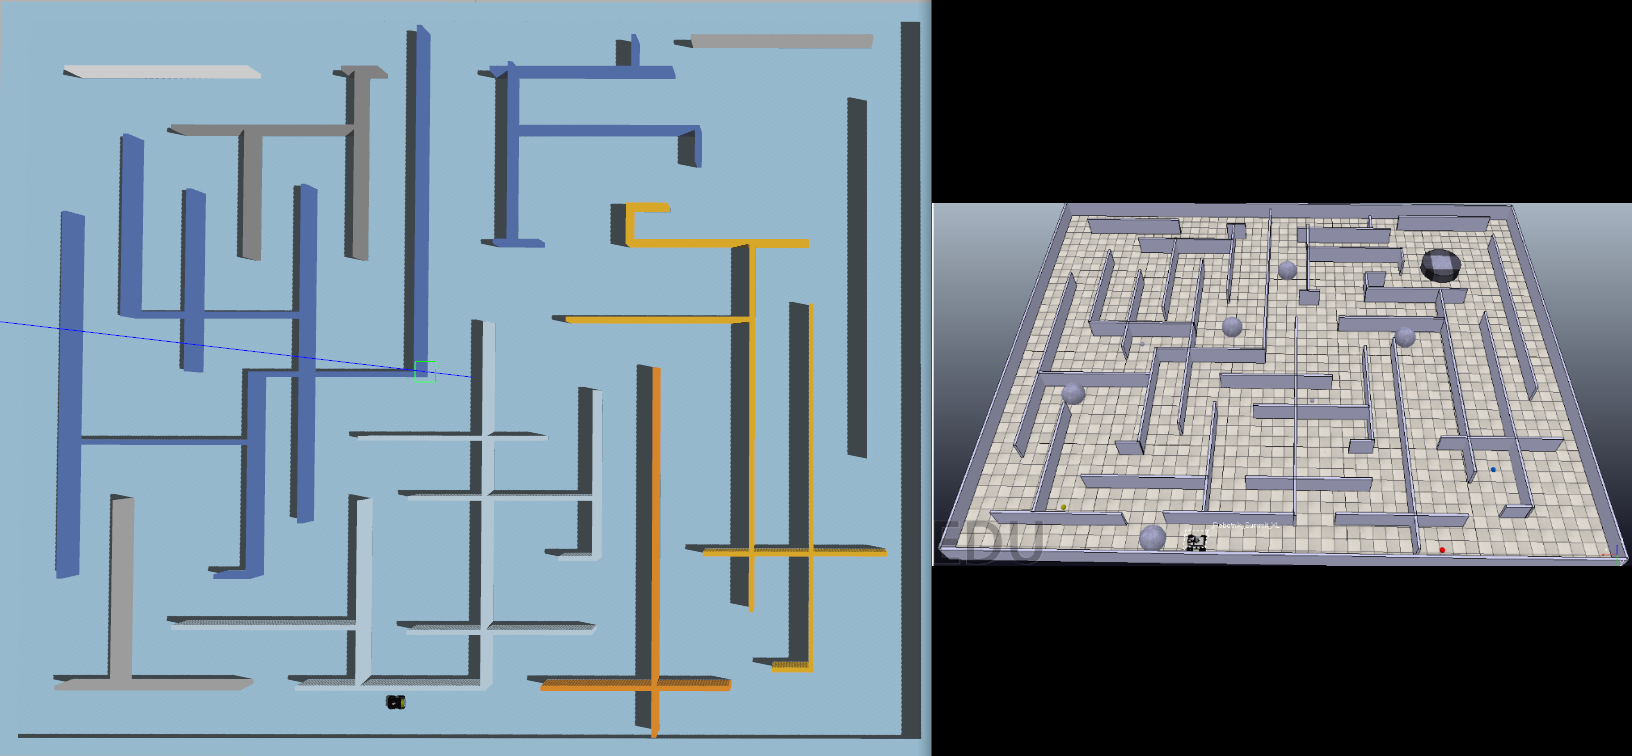
\includegraphics[scale=0.18]{figuras/world_compare.png}                   
                    \caption{Reconstrução do Labirinto}
                    \label{}                    
                \end{figure}
                \begin{itemize}
                    \item Como Foi Desenvolvido;
                    \item Desenvolvimento do launcher. 
                \end{itemize}              
                           
            \end{frame}
            
        \subsection{Desenvolvimento}

            \begin{frame}{Desenvolvimento}
                \begin{figure}[htb]
                    \centering
                    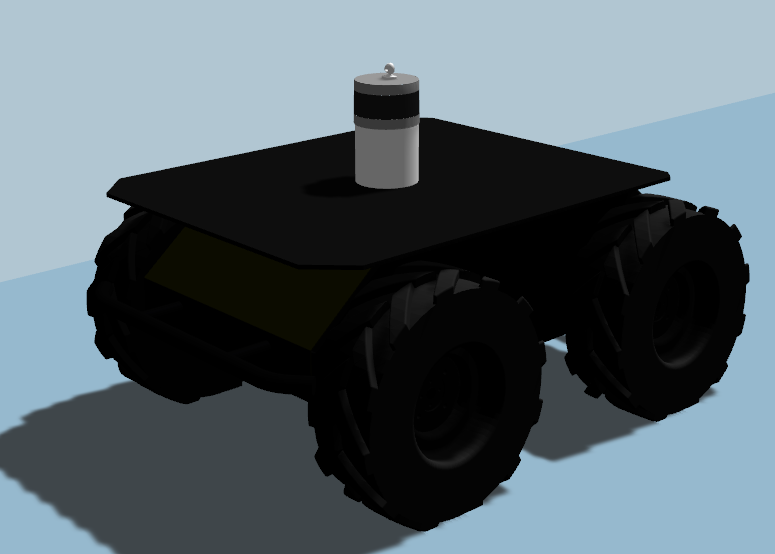
\includegraphics[scale=0.35]{figuras/husky.png}                   
                    \label{}
                    \caption{Husky no Gazebo}
                \end{figure}

            \end{frame}

            \begin{frame}{Desenvolvimento}
                \centering              
                    \begin{figure}[htb]
                        \centering
                        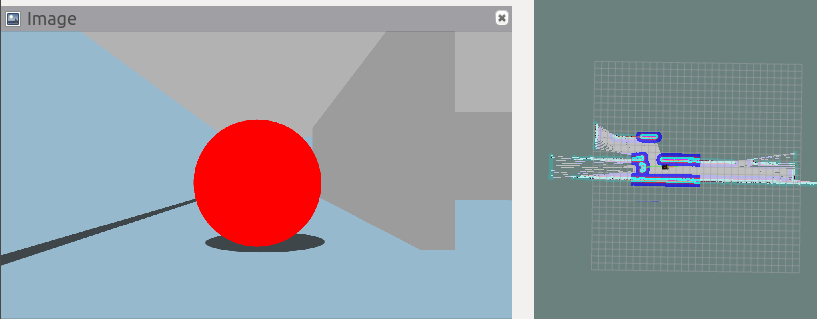
\includegraphics[scale=0.35]{figuras/detection_and_mapping.png}                   
                        \label{}
                        \caption{Mapeamento e Detecção}
                    \end{figure} 
            \end{frame}

            \begin{frame}{Desenvolvimento}
                \centering
                    \begin{figure}[htb]
                        \centering
                        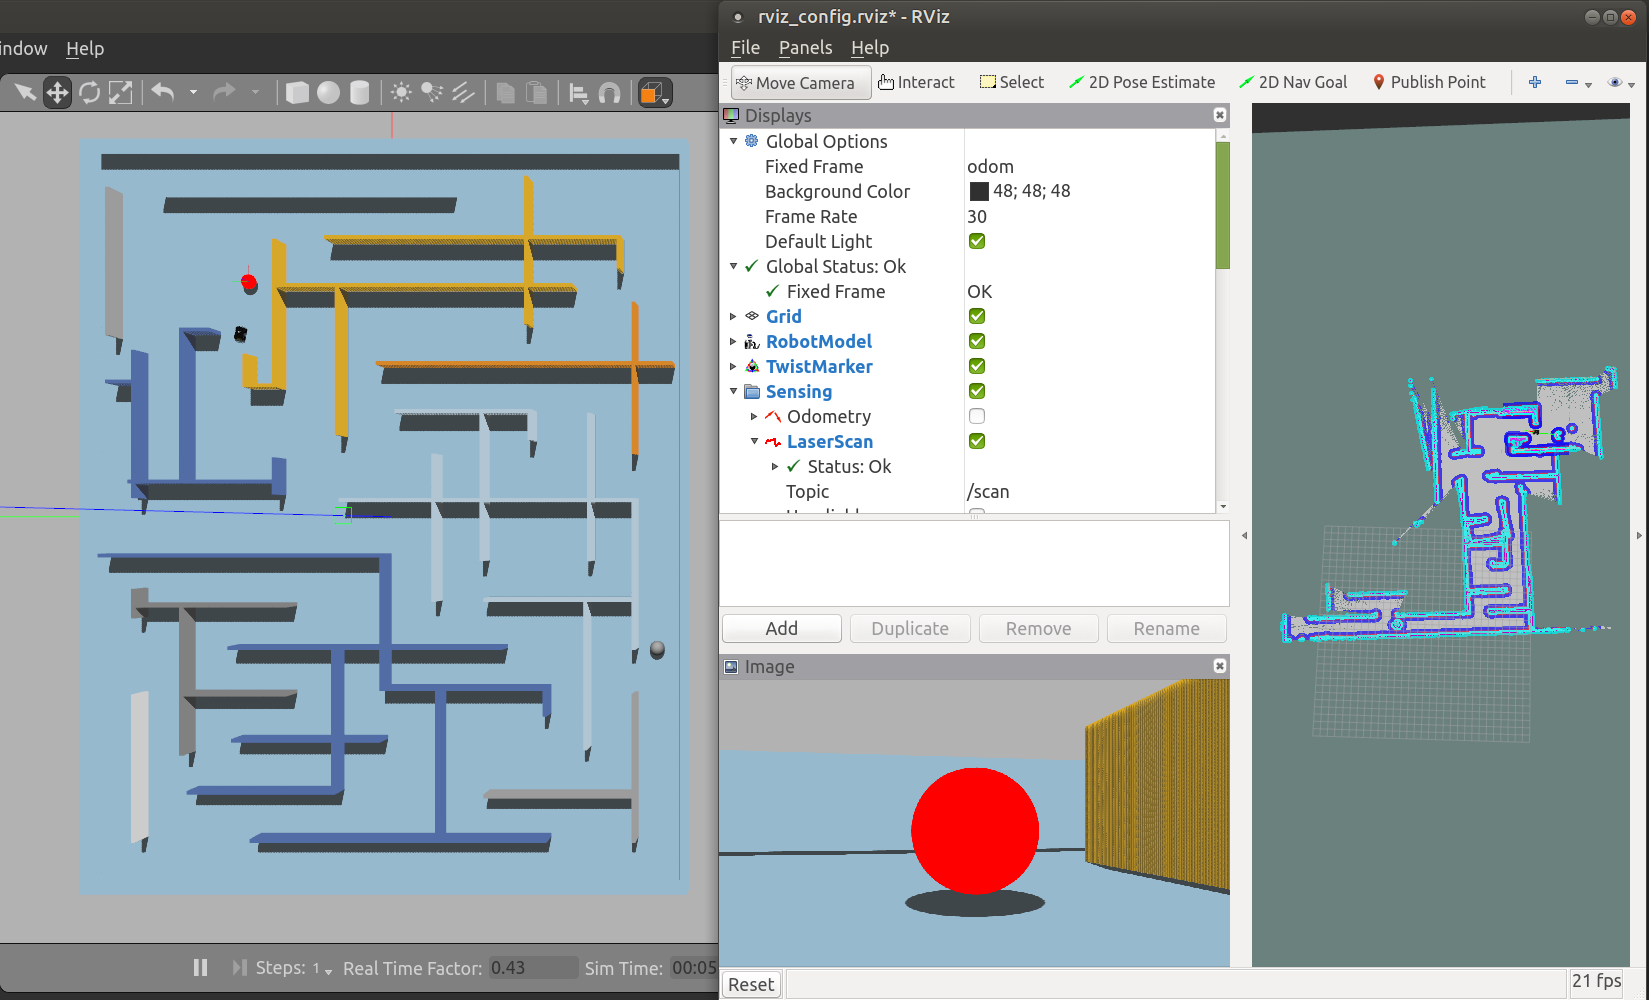
\includegraphics[scale=0.18]{figuras/simulation.png}                   
                        \label{}
                        \caption{Simulação}
                    \end{figure}                 
            \end{frame} 

            \begin{frame}{Simulação}
                \centering
                     \movie[width=320px, height=180px]{Video}{video/challenge_1_new_world.mp4}                                  
            \end{frame} 

           
            
            \begin{frame}{Agradecimento}
                \centering Obrigado           
            \end{frame}

\end{document}
